\subsection{Test 2}
\begin{enumerate}
	\item Consider the function $f(x,y) = x^2-2x+y^2-4y+7$.\\
	\begin{enumerate}[a.]
		\item Find equations for an plot (if possible) the C-level curves of $f$ for $C=3$ and $C=1$.\\
		\indent
		We will try to find the level curve for any $C$ and then plug in 1 and 3.\\
		$x^2-2x+y^2-4y+7=C$\\
		$x^2-2x+1+y^2-4y+4=C-2$\\
		$(x-1)^2+(y-2)^2=C-2$: A circle of radius $\sqrt{C-2}$ centered at $(1,2)$.\\
		For $C=1$, the level curve does not exist because the circle would have a radius of $\sqrt{2-1}=\sqrt{-1}$.\\
		For $C=3$, the level curve is $(x-1)^2+(y-2)^2=1$.
		
		\begin{figure}[h]
			\centering
			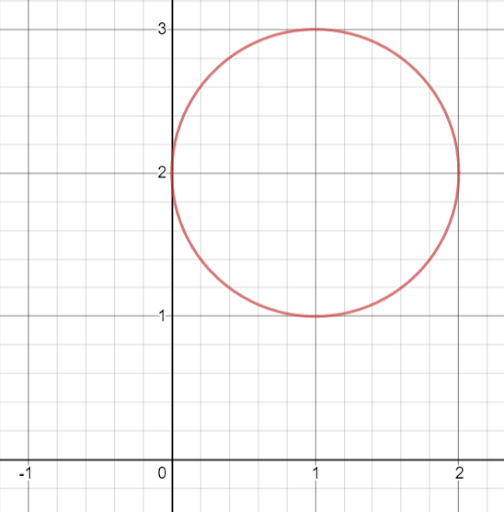
\includegraphics[scale=.24]{Images/additionalMaterials/test2_circle}
		\end{figure}
		
		\item Compute $\nabla f$.\\
		\indent
		$\nabla f = \langle f_x, f_y\rangle=\langle 2x-2,2y-4\rangle$\\
		
		\item Find the equation of the plane tangent to the surface $z=f(x,y)$ at the point $(x_0,y_0,z_0)=(2,4,7)$.\\
		\indent
		$\vec{n}=\langle f_x, f_y, -1\rangle=\langle 2x-2, 2y-4, -1\rangle$\\
		At $(2,4,7)$, $\vec{n}=\langle 2,7,-1\rangle$.\\
		So, the plane equation is $\langle 2,7,-1\rangle\cdot\langle x-2, y-4, z-7\rangle=0$.\\
		
		\item Perform one iteration of gradient descent on $f(x,y)$ with a learning rate $delta = 1/4$ starting from the point $(x_0,y_0)=(2,4)$.\\
		\indent
		$(x_n,y_n)=(x_{n-1},y_{n-1})-\delta\nabla f$\\
		$(x_0,y_0)=(2,4)$,$\delta=1/4$, and $\nabla f=\langle 2x-2,2y-4\rangle$\\
		$(x_1,y_1)=(2,4)-\frac{1}{4}\langle 2(2)-2, 2(4)-4\rangle$\\
		$=(3/2, 3)$\\
	\end{enumerate}

	\item Recall that for a differentiable function $f(x,y)$ and the unit vector $\hat{u}=\langle a,b\rangle$, we proved that $D_{\hat{u}}f=\nabla f\cdot\hat{u}$.
	\begin{enumerate}[a.]
		\item Prove the statement "The gradient is the direction of steepest ascent" by showing that the directional derivative $D_{\hat{u}}f$ is maximized when $\hat{u}\parallel\nabla f$.\\
		\indent
		$D_{\hat{u}}f=\nabla f\cdot\hat{u}=\norm{\nabla f}\norm{\hat{u}}\cos{\theta}=\norm{\nabla f}\cos{\theta}$\\
		This value is maximized when $\theta$ is a multiple of $2\pi$, meaning that the angle between $\nabla f$ and $\hat{u}$ is 0. This means that the maximum value of the directional derivative, the direction of steepest ascent, is in the same direction as $\nabla f$.\\
			
		\item State the limit definition of the directional derivative $D_{\hat{u}}f$. Starting from that definition, prove that $D_{\hat{u}}f=\nabla f\cdot\hat{u}$.\\
		$D_{\hat{u}}f=\lim_{h\to 0}{\frac{f(x+ah,y+bh)}{h}}$ and $\hat{u}=\langle a,b\rangle$.\\
		$=\lim_{h\to 0}{\frac{f(x+ah,y+bh)-f(x+ah,y)}{h}+\frac{f(x+ah,y)-f(x,y)}{h}}$\\
		$=b\lim_{h\to 0}{\frac{f(x,y+bh)-f(x,y)}{bh}}+a\lim_{h\to 0}{\frac{f(x+ah,y)-f(x,y)}{ah}}$\\
		$=bf_y+af_x=\langle f_x, f_y\rangle\cdot\langle a,b\rangle=\nabla f\cdot\hat{u}$\\
	\end{enumerate}
	
	\item Use the method of Lagrange Multipliers to find the maximum of the product of two numbers $x$ and $y$ given that $(x,y)$ is a coordinate pair in the 1st quadrant located on the unit circle centered at the origin. Begin by stating the objective function $f(x,y)$ and the constraint equation $g(x,y)=k$.\\
	\indent
	Objective Function: $f(x,y)=xy$\\
	Constraint Equation: $g(x,y)=x^2+y^2=1$, $x\geq 0$ and $y\geq 0$.\\
	$F(x,y,\lambda)=xy+\lambda(1-x^2-y^2)$\\
	$\frac{\partial F}{\partial x}=y-2\lambda x$, $\frac{\partial F}{\partial y}=x-2\lambda y$, and $\frac{\partial F}{\partial\lambda}=1-x^2-y^2$.\\
	$\langle y-2\lambda x,x-2\lambda y,1-x^2-y^2\rangle=\vec{0}$\\
	$\begin{cases}
		y=2\lambda x \\
		x=2\lambda y \\
		x^2+y^2=1
	\end{cases} 
	\implies
	\begin{cases}
		\lambda = 1/2 \\
		x = 1/\sqrt{2} \\
		y = 1/\sqrt{2}
	\end{cases}$\\
	So, the maximum product is $\frac{1}{\sqrt{2}}\cdot\frac{1}{\sqrt{2}}=\frac{1}{2}$ at $\left(\frac{1}{\sqrt{2}},\frac{1}{\sqrt{2}}\right)$\\
	
	\item The function $p(x,y)=\frac{1}{\pi}\exp{\left(-(x-a)^2-(y-b)^2\right)}$ is the probability density function of a bivariate normal distribution with mean $(a,b)$ and standard deviation $\frac{1}{\sqrt{2}}$. Show that the global maximum of $p(x,y)$ occurs at $(a,b)$.\\
	\indent
	$p_x=\frac{1}{\pi}(-2(x-a))\exp{(-((x-a)^2+(y-b)^2))}$\\
	$p_y=\frac{1}{\pi}(-2(y-b))\exp{(-((x-a)^2+(y-b)^2))}$\\
	$p_x=0$ when $x=a$ and $p_y=0$ when $y=b$\\
	$\implies (a,b)$ is a critical point.\\
	$p_{xx}=\frac{1}{\pi}(-2(y-b))\exp{(-((x-a)^2+(y-b)^2))}-2\exp{(-((x-a)^2+(y-b)^2))}$\\
	$=\frac{1}{\pi}(4(x-a)^2-2)\exp{(-((x-a)^2+(y-b)^2))}$\\
	Similarly, $p_{yy}=\frac{1}{\pi}(4(y-b)^2-2)\exp{(-((x-a)^2+(y-b)^2))}$\\
	$p_{xy}=p_{yx}=\frac{4}{\pi}(x-a)(y-b)\exp{(-((x-a)^2+(y-b)^2))}$\\
	$p_{xx}(a,b)=\frac{-2}{\pi}$, $p_{yy}(a,b)=\frac{-2}{\pi}$, and $p_{xy}(a,b)=p_{yx}(a,b)=0$\\
	$H(a,b)=\begin{bmatrix}
		\frac{-2}{\pi} & 0 \\
		0 & \frac{-2}{\pi}
	\end{bmatrix}$\\
	$\det{(H(a,b))}=\frac{4}{\pi^2}$\\
	$(a,b)$ is an extrema because $\det{(H(a,b))}>0$.\\
	Since $f_{xx}(a,b)<0$ and $f_{yy}(a,b)<0$, $(a,b)$ is a maximum.\\
	$(a,b)$ is a global maximum because $p(x,y)$ is strictly decreasing as you move away from $(a,b)$.\\
	
	\item Let the C-level curve of the function $f(x,y)$ be parameterized by the VVF $\vec{r}(t)=\langle x(t), y(t)\rangle$. Use the chain rule to show that $\nabla f(\vec{r}(t))\perp\vec{r^\prime}(t)$ for all $t$.\\
	\indent
	Since $\vec{r}(t)$ parameterizes a C-level curve of $f$, $f\circ\vec{r}(t)=C$. Where $C$ is a constant.\\
	$\frac{\mathrm{d}}{\mathrm{d}t}(f\circ\vec{r}(t))=\frac{\mathrm{d}}{\mathrm{d}t}C$\\
	$\frac{\partial f}{\partial x}\frac{\mathrm{d}x}{\mathrm{d}t}+\frac{\partial f}{\partial y}\frac{\mathrm{d}y}{\mathrm{d}t}=0$\\
	$\left<\frac{\partial f}{\partial x},\frac{\partial f}{\partial y}\right>\cdot\left<\frac{\mathrm{d}x}{\mathrm{d}t},\frac{\mathrm{d}y}{\mathrm{d}t}\right>=0$\\
	$\nabla f(\vec{r}(t))\cdot\vec{r^\prime}(t)=0$\\
	$\implies \nabla f(\vec{r}(t))\perp\vec{r^\prime}(t)$\\
\end{enumerate}